\section{Implementation}

\subsection{Managing team analytic states}
% 
% visualization state
% Shrinivasan2008b discusses managing visualization states in an analytic process


A particular challenge in implementing CAnalytics is effective management of dynamic states that occur throughout the information analysis process. Rather than simply displaying a static set of data as in many visualization systems, data and views in CAnalytics keep updating as analysts collect evidence, re-arrange views, and develop hypotheses. Each change generates a new ``state'' in the analytic system, which is like a ``shot'' of system dynamics that determine how a
system looks like. Managing the dynamically changing states is particularly important in collaborative analysis as states of all analyst's system should always keep synchronized; otherwise, a coordination breakdown could occur. 

\begin{figure}
	\centering
	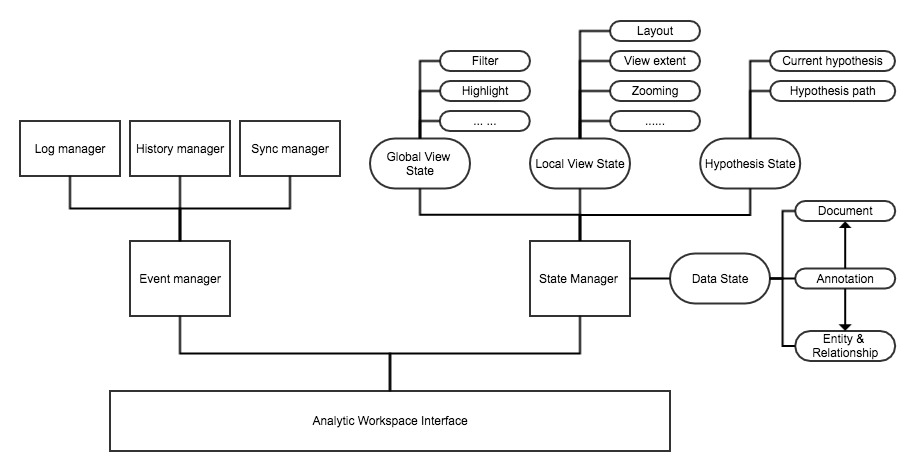
\includegraphics[width=\columnwidth]{03-System/img/architecture.jpg}
	\caption{State management in a dynamic system.\label{fig:architecture}}
\end{figure}

Aligned with the three major activities in information analysis, we create state managers for each activity, as shown in Figure~\ref{fig:architecture}. A data manager is in charge of the raw documents, user-created entities and relationships, and annotations that indicate in which part of a document is an entity created. A view manager controls the contemporary visualization state in the system. It includes a global view state and a local view state. The global state controls factors that affect all the views in the system. For example, a filter applies to all views so that the same subset of data is shown across views. A highlight determines which entities are on focus and underscore them in their representation. A local view state manages how the data looks like in each individual visualization, including the position of the view in the workspace, the view extent, the zooming level, etc. 
Finally, the hypothesis state manager controls the current active hypothesis, as well as a path of hypotheses it builds upon. The path keeps track of the development of hypotheses and enables analysts to trace back. 


\begin{figure}
	\centering
	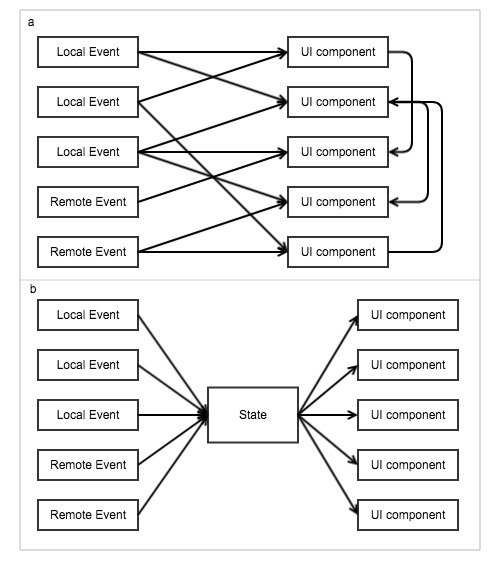
\includegraphics[width=.4\linewidth]{03-System/img/state_management.jpg}
	\caption{Diagrams showing two state management approaches. a) Event-driven approach: each interface component manages its own state and updates itself driven by events. b) Our approach: a central state manager takes care of all events and notifies interface components whenever there is a need to update.\label{fig:state_management}}
\end{figure}

User interactions drive the change of system states. These interactions are modeled as events and controlled by a manager. Depending on the type of events, the system includes a log manager, which saves events as system logs and team activity history, and a sync manager, which broadcasts events to the other systems in the team. 

After defining state managers and event managers, another challenge is to connect them to function as a dynamic system. A common implementation is event-driven:
each system component manages its own state and subscribes to events that change its state. This approach works for simple applications, but may be difficult to scale up in a complex system, especially a collaborative system in which there exist multiple sources that could change the system states. As shown in Figure~\ref{fig:state_management}a, a local
component can be changed by both a local (the user in operation) and a remote interaction (teammate). In turn, the
change of the local component could cause a change to another local component or
even a remote component. For example, a brushing interaction on the network changes
the state of the network (highlight entity nodes). The change of network state
in turn causes change to other views, for example, a reduced data view in the
map showing related locations to those highlighted entities. The state could
also be changed by a remote interaction when collaborators are sharing their
view, and, similarly, cause change to other views. To some extent, the groupware
developer no longer understands what changes a view, and the state of the
groupware would become out of control.

To address the issue, we employed a state-centered approach to make state control more structured and
clear. As Figure~\ref{fig:state_management}b shows, an event manager takes control of all events, whether
they are local or remote events. The event manager dispatches events to
different event handlers and makes changes to a central state manager. Whenever
the state changes, the state manager sends a signal to related interface
components, notifying them to update the view. This approach centralizes the
management of states, and the central state becomes the ``single source of truth'' \footnote{Single source of truth: \url{https://en.wikipedia.org/wiki/Single_source_of_truth}}. 
All user interfaces (including the ad hoc user and teammates) subscribe to \emph{the} state so that they will always be consistent. 

A typical event flow is demonstrated in Figure~\ref{fig:flow}. An event is triggered by a user
interaction. The event is sent to the Event Manager for processing. Depending on the nature of the event, the event manager may do three things. The event could change the local state directly (could be data, view, and hypothesis). The event is also sent to the history manager. It is saved as a system log for research purposes. There are also a set of rules that decide if the event is of interest to analysts. If it is, it is also saved as part of team history. Finally, the event is also passed to the sync manager if considered necessary. The sync manager then broadcasts the event to other systems in the team so that it can make exactly the same change in their state. 



\begin{figure}
	\centering
	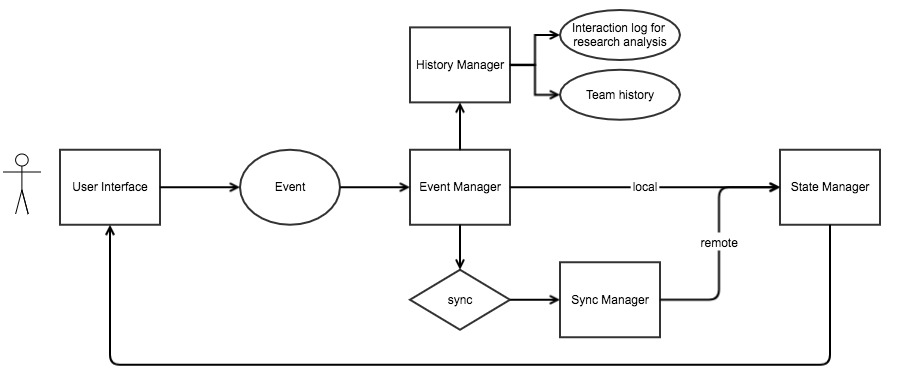
\includegraphics[width=\columnwidth]{03-System/img/flow.jpg}
	\caption{Event flow in a collaborative system.\label{fig:flow}}
\end{figure}

The system employs a standard three-layer web application architecture. The frontend is the application running in a browser that end users interact with directly. It is implemented in Javascript and HTML. We use PostgreSQL as the database. The backend server is implemented in Python/Django and Node.js. The Django server takes care of most REST API requests and reads and writes data into database. The Node.js is responsible for broadcasting data to systems in a team so that they can communicate with each other and keep their system state consistent. 
The tool takes advantage of the state-of-the-art HTML5 WebSocket technique to
realize real-time communication. WebSocket is a bidirectional, full-duplex
communication channel that operates through a single socket over the web. It is
part of HTML5 and provides a true standard for building scalable, real-time web
applications. Since most modern browsers implement the protocol as a standard,
no plug-in or other installation is required, which ensures convenient
accessibility to users. We intentionally keep the API server and sync server separate so that they are loosely coupled. Each server works on its own (the Django server will be like a single-user application on its own, and the Node server can be potentially plugged into other applications to enable collaboration). This approach opens an opportunity to develop the Node server into a \emph{service} that provides a more general collaborative functionality to standalone applications in the future. 

\subsection{Conflict resolution}

An important consideration in supporting collaboration is conflict resolution. A potential issue in CAnalytics is the addition of multiple annotations to the same text. CAnalytics supports multiple annotations by stacking them and marking the author and creation time of each annotation. The same issue may exist when users add multiple relationships to two entities. The node-link graph in CAnalytics resolves the issue by displaying multiple labeled links between two nodes (as in the node-link graph in Figure~\ref{fig:interface}). Therefore analysts can identify the potential conflicts and try to resolve them. It is also possible that it does not conflict at all. It may be two possible hypotheses due to uncertainty. In either case, this approach helps analysts identify potential issues. 

\subsection{View restoration and sharing}
Views in CAnalytics are handled as global views and local views. Global views refer to the window of each visualization, including which windows are open, the size of the window, and its position. Global views are saved and shared in JSON format. 

Local views are more complicated as they include all the nodes and paths of visualization. To restore the view back to the same layout when the analyst reopens it, positions of all individual nodes are saved. This means a large amount of data will potentially be downloaded and parsed when individuals intend to restore an existing view. This is still fine (though it probably would take a longer time), yet presents a challenge for real-time sharing. If we share the whole view state node by node in real-time, we need to pass a lot of data for each frame, and several frames per second for smooth animation. Obviously, this is not optimal. Instead of state sharing, we adopt event sharing. Only attributes of an event, for example, type of event (e.g. 'click', 'scroll'), the target of the event (which node is the event applied to), are shared. When partners receive the event, the event is applied to the visualization. Since each event has a deterministic effect, the partner will see the same animation and result of the visualization as the event source. By sharing only event and ensuring event effects are deterministic, we make possible real-time view sharing a smooth experience.